\section{Introduction to CSPs}\label{sec:intro}

Constraint Satisfaction Problems (CSPs) represent a versatile and powerful area of study, offering a general framework that can be applied to a myriad of domains—from logistics and scheduling to artificial intelligence and financial optimization. The true strength of CSPs lies in their generality; new problems from developing fields can often be translated into CSPs, allowing one to leverage a wealth of mature, efficient solver technologies. CSPs are an indispensable tool for modeling complex systems with interacting variables with restrictions. For a good, thorough reference on the subject, see \citep{rossi2006handbook} and \citep{tsang1993foundations}.

\subsection{What CSPs Are}\label{sec:csp-def}

A CSP is fundamentally built out of a set of generating relations over a domain $d$. A CSP starts with a finite set of \say{atomic relations}, each with a fixed arity. A relation of arity $n$ can be defined as any set of $n$-tuples of elements of $d$. These atomic relations serve as the building blocks for defining more complex relations within the CSP. Such construction is achieved through \say{relational composition}, a process involving conjunction and existential quantification over shared variables. For instance, given relations $R_1(x,y)$ and $R_2(y,z)$, a new relation can be defined as

\begin{equation}\label{equation:relation-composition-example}
R_3(x,z) := \exists y. R_1(x,y) \wedge R_2(y,z).
\end{equation}

It should be noted that we allow variables to be freely deleted, duplicated, and equated as part of relational definitions. An algebra of relations closed under relational composition is called a \say{relational clone}. A familiar example is linear programming, where atomic relations like $x+y\leq z$ and $x=y$ can be composed to form more intricate linear systems. In that example, the variable domain might be the set of rationals.

Given a CSP, an instance of this CSP consists of the following:

\begin{itemize}
  \item $X$: a finite set of variable symbols.
  \item $C$: a finite set of constraints (called "clauses") consisting of expressions of the form $R(x_1,x_2,...,x_n)$, where $R$ is an $n$-ary, atomic relation from our CSP, and $x_i \in X$, for all $i$.
\end{itemize}

An assignment of an instance consists of a map from $X$ into $d$, and the truth value (or valuation) of an instance relative to an assignment is the evaluation of the conjunction of all constraints with respect to the assignments. If an assignment produces a true valuation, then, the instance is said to be "satisfiable", and the assignment is called a "satisfying assignment" for that instance. One may interpret the satisfiability of CSP instances as the 0-ary relations definable within the CSP.

\begin{remark}\label{remark:instance-terminology}
Not all authors make a clear distinction between CSPs and their instances. Some will refer to CSP instances as just "CSPs". Research on CSP complexity is consistent in making this distinction, while research on distributed CSPs is not. We've decided to be clear, as confusion may arise if a distinction is not made. One does not need a fixed set of variables to define the CSPs describing linear programming or boolean satisfiability, for example, while one does need a fixed set of variables to define their instances.
\end{remark}

\begin{remark}\label{remark:relational-database-terminology}
There is a close relationship between relational database theory and the theory of CSPs. This connection will not be emphasized here, but some terminology from this link should be noted. Rarely, a CSP will, itself, be called a "database", as, in the finite domain case, it is the same thing as a relational database. What's more common is the usage of the word "query" to describe CSP instances, which one will most often see in the field of constraint programming.
\end{remark}

\subsection{Example: Boolean Satisfiability}\label{sec:two-sat}

By far the most well-studied CSPs are from the domain of boolean satisfiability. Each problem has the same domain; the booleans, 0 and 1. There are several versions of the problem. The simplest is called 2-SAT and consists of three binary relations, $x \vee y$, $\neg x \vee y$, and $\neg x \vee \neg y$. By commutativity, we can also define $x \vee \neg y$ as $\neg y \vee x$. An instance of a boolean satisfiability problem will generally be a formula in conjunctive normal form. As an example, we have the following instance;

\begin{equation}\label{equation:two-sat-example-pt1}
    (x_1 \lor \neg x_2) \land (\neg x_1 \lor x_3) \land (x_2 \lor \neg x_3) \land (\neg x_1 \lor \neg x_2)
\end{equation}

We can note that this instance has three variables, $x_1$, $x_2$, and $x_3$. 2-SAT is a tractable CSP, meaning we can always efficiently calculate if a solution exists and what it is if it does. 

\begin{remark}
    When we describe something as "efficient" to solve, we always mean that it can be solved in polynomial time.
\end{remark}

The standard reasoning method for 2-SAT is called binary resolution and states that;

\begin{equation}\label{equation:binary-resolution}
\frac{C_1 \lor p \quad C_2 \lor \neg p}{C_1 \lor C_2}.
\end{equation}

This allows us to derive new clauses from the old ones by connecting them with shared variables of opposite polarity. We can, in particular, apply it to the clauses $x_1 \lor \neg x_2$ and $\neg x_1 \lor \neg x_2$, allowing us to derive $\neg x_2 \lor \neg x_2 = \neg x_2$. This tells us that $x_2$ must be $0$. Substituting this into our original problem and simplifying leads to

\begin{equation}\label{equation:two-sat-example-pt2}
(\neg x_1 \lor x_3) \land \neg x_3
\end{equation}

We can clearly see that $x_3$ must be $0$ since it appears negated and alone within a clause. Making this observation and substituting the implied value is called "unit propagation".
% , something we will speak about in more detail in section \ref{sec:arc-consistency}. 
By doing this, we end up with

\begin{equation}\label{equation:two-sat-example-pt3}
\neg x_1
\end{equation}

forcing $x_1$ to be $0$. Ultimately, we conclude that this problem has a satisfying instance, that being the map $\langle x_1 \rightarrow 0; x_2 \rightarrow 0; x_3 \rightarrow 0\rangle$.

While it's convenient to work with 2-SAT, it is not very expressive. Most boolean SAT solving is done using at least 3-SAT. This version of the problem has the relations, $x \vee y \vee z$, $\neg x \vee y \vee z$, $\neg x \vee \neg y \vee z$, and $\neg x \vee \neg y \vee \neg z$.

Solvers often do not enforce a specific argument number. If we need to express a clause in 3-SAT that has more than three clauses, we can split it up by introducing dummy variables. For example,

\begin{equation}\label{equation:three-sat-split-pt1}
\neg x_1 \vee \neg x_2 \vee \neg x_3 \vee x_4 \vee x_5
\end{equation}

can be defined as

\begin{equation}\label{equation:three-sat-split-pt1}
\exists d_1, d_2. (\neg x_1 \vee \neg x_2 \vee d_1) \wedge (\neg d_1 \vee \neg x_3 \vee d_2) \wedge (\neg d_2 \vee x_4 \vee x_5)
\end{equation}

by applying binary resolution, we can recover the original formula from its 3-SAT rendition. A similar procedure cannot be used to turn a 3-SAT formula into a 2-SAT formula, indicating a true jump in complexity. One does not gain meaningful expressiveness for N-SAT beyond N=3.

There does not exist a known method to efficiently solve 3-SAT problems, and it's strongly believed that such a method cannot exist. 3-SAT is, perhaps, the Ur-Example of a complete, hard problem. It is NP-complete, meaning that any problem whose solution is efficiently verifiable can be efficiently expressed as a 3-SAT problem. This also means that it is at least as hard as the hardest of such problems, since, if 3-SAT can be solved efficiently, then all problems efficiently expressible in 3-SAT can as well. It is also known that all finite-domain CSPs are, at worst, NP-hard, meaning they can all be efficiently translated into 3-SAT. 3-SAT is only one of infinite many NP-complete finite domain CSPs; see section \ref{sec:polymorphisms} for more details on this.

Despite its theoretical difficulty, much practical progress has been made. There are a wide variety of methods that can solve special cases quite efficiently. Research into 3-SAT is one of the most active areas in computer science, and for good reason. Its flexibility means that industrial benefits from solver improvements can have wide-reaching consequences.

See the handbook \citep{biere2009handbook} for reference.

\subsection{Example: Diophantine Equations}\label{sec:diophantine}

Diophantine Equations are an interesting example of a CSP with, in some sense, maximal expressiveness. It is generated from all polynomial equations over the domain of the integers. The most famous example of such a polynomial is the equation at the center of Fermat's Last Theorem, now known to have no satisfying positive assignments.

\begin{equation}
    x^3 + y^3 = z^3
\end{equation}

By Matii︠a︡sevich's theorem, we know that Diophantine Equations are Turing complete. This means that all computable relations are expressible as some system of Diophantine Equations. For example, despite exponentiation between two variables not being a polynomial, such a relation is definable as a system of polynomials, though the construction is quite involved \citep{matii︠a︡sevich1993hilbert}. This expressiveness implies that solving Diophantine Equations, in general, is as hard as solving the hardest possible problem, since that problem can be expressed as a system of Diophantine Equations.

\begin{remark}\label{remark:natural-mat}
Matii︠a︡sevich's theorem was actually proven over the domain of natural numbers, that is the non-negative integers, including 0. The version over the integers is a simple corollary since an integer, $n$, can be restricted to be a natural number using the expression $\exists i_1, i_2, i_3, i_4. n = i_1^2 + i_2^2 + i_3^2 + i_4^2$, by Lagrange's four-square theorem. Such expressions can be added to any system of polynomials over the naturals to create a system over the integers defining the same relation.
\end{remark}

Diophantine Equations are an example of an infinite-domain CSP. They are also an example where instances are generally undecidable. That is, one cannot, in general, even know if a solution exists, even with infinite effort. They are, however, semi-decidable. That is, we can define an algorithm that will find a solution if one exists but may run forever if a solution does not exist. This can be done by counting through tuples of assignments (using some pairing function to define a canonical ordering \citep{rosenberg2003efficient}), and evaluating the system of polynomials at each assignment. This will always tell you if the assignment is satisfying in finite time, meaning that, if a solution exists, it will eventually be found by this procedure.

See \citep{matii︠a︡sevich1993hilbert} for reference.

\subsection{Example: Three Coloring}\label{sec:three-coloring}

Graph three coloring is a common example used to introduce CSPs to new audiences. The goal is to color the nodes of a graph with three colors such that no two same-colored nodes touch. The CSP itself consists of a single binary relation asserting the inequality between three elements, typically named after primary colors.

\begin{equation}\label{equation:three-color-neq-def}
    \neq\ = \{ (Blue, Red), (Blue, Green), (Red, Blue), (Red, Green), (Green, Blue), (Green, Red) \}
\end{equation}

Graphs become instances by translating edges into binary relations. Take this graph as an example;

\begin{center}
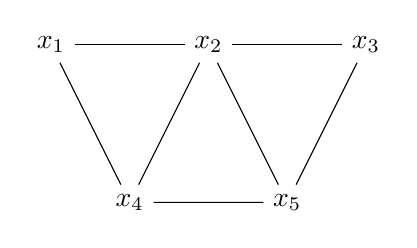
\begin{tikzpicture}
  \node (A) at (0,0) {$x_1$};
  \node (B) at (2,0) {$x_2$};
  \node (C) at (4,0) {$x_3$};
  \node (D) at (1,-2) {$x_4$};
  \node (E) at (3,-2) {$x_5$};

  \draw (A) -- (B) -- (C);
  \draw (A) -- (D) -- (E) -- (C);
  \draw (D) -- (B);
  \draw (E) -- (B);
\end{tikzpicture}
\end{center}

We can simply list the edges using the inequality relation to produce the corresponding CSP instance;

\begin{equation}
    x_1 \neq x_2 \wedge x_1 \neq x_4 \wedge x_2 \neq x_3 \wedge x_2 \neq x_4 \wedge x_2 \neq x_5 \wedge x_3 \neq x_5 \wedge x_4 \neq x_5
\end{equation}

A solution to the graph coloring problem is then an assignment of colors that satisfies the instance. 

If we think about the structure of this graph, we notice that it has three triangles, the left and right side triangles $(x_1, x_2, x_4)$  and $(x_2, x_3, x_5)$, and the central triangle $(x_2, x_4, x_5)$. Each must be a triple of distinctly colored points. The edge between $x_4$ and $x_5$ forces those two to have distinct colors, while the two side triangles share a color at $x_2$. These two observations force us to conclude that the left triangle has the colors of the right triangle flipped along the bisector going through $x_2$. If we arbitrarily select $x_1$ to be $Blue$ and $x_2$ to be $Red$, we are then forced into the coloring;

\begin{equation}
 \langle x_1 \rightarrow Blue; x_2 \rightarrow Red; x_3 \rightarrow Green; x_4 \rightarrow Green; x_5 \rightarrow Blue\rangle,
\end{equation}

which will satisfy this instance. We can place these colors back on the graph to verify the solution visually.

\begin{center}
\begin{tikzpicture}
  \node (A) at (0,0) {${\color{blue}\CIRCLE}$};
  \node (B) at (2,0) {${\color{red}\CIRCLE}$};
  \node (C) at (4,0) {${\color{darkgreen}\CIRCLE}$};
  \node (D) at (1,-2) {${\color{darkgreen}\CIRCLE}$};
  \node (E) at (3,-2) {${\color{blue}\CIRCLE}$};

  \draw (A) -- (B) -- (C);
  \draw (A) -- (D) -- (E) -- (C);
  \draw (D) -- (B);
  \draw (E) -- (B);
\end{tikzpicture}
\end{center}

Like 3-SAT, graph coloring is an NP-complete problem. However, translating problems into graph coloring is often more clunky and non-intuitive than 3-SAT, and solving methods are far less developed. But this problem has similar broad applicability for expressing a wide variety of problems. For example, the original proof that zero-knowledge proofs exist was based on graph coloring \citep{Numberphile2ZKP}.

\begin{remark}\label{remark:graph-map}
The original ZKP setup is usually described in terms of map coloring rather than graph coloring; though, this is merely a different way to draw the same problem. Formally, a map, in this sense, is defined to be a loopless, planar graph.
\end{remark}

\subsection{Multi-domain CSPs}\label{sec:multidomain}

In some applications, CSPs may have multiple domains. An example of this is mixed-integer linear programming, which has variables ranging over integers, rationals, or booleans, and relations sensitive to each of these domains. A multi-domain CSP will, instead of having a single domain, have a set of domain sets, $D$. Additionally, for each $n$-ary relation, $R$, we will have a tuple $T^R \in D^n$ indicating the domain of each argument.

Instances for multi-domain CSPs can be defined as

\begin{itemize}
  \item $X$: a finite set of variables
  \item $d$: a function mapping $X$ to $D$
  \item $C$: a finite set of constraints (called "clauses") consisting of expressions of the form $R(x_1,x_2,...,x_n)$, where $R$ is an $n$-ary, atomic relation from our CSP, and $x_i \in X$ and $d(x_i) = T^R_i$, for all $i$
\end{itemize}

Assignments can be extended to this setup in a natural way, as a dependent map from $x \in X$ to $d(x)$.

It’s worth noting that multi-domain CSPs can be seen as special cases of single-domain CSPs. The single-domain CSP will have $\bigcup D$ as its domain. We can forget $T^R$ and treat each relation from the multi-domain CSP as a relation over $\bigcup D$. If need be, we can add predicates to the CSP indicating which set of $D$ the argument initially came from, allowing one to restrict the domain of variables; though this is usually unnecessary as domains will already be restricted by the relations those variables appear in. This construction illustrates that we don’t gain expressiveness when moving from single to multi-domain CSPs; although keeping domains separated may still be pragmatic for the purposes of implementation.

\subsection{CSPs and Graph Homomorphisms}\label{sec:homomorphism}

Graph homomorphisms are the notion of structure-preserving map between graphs. 

\begin{definition}
A graph, for our purposes, is a set of vertices, $V$, and a set of ordered pairs of $V$s, $E$, representing edges.
\end{definition}

\begin{definition}
A graph homomorphism from a graph $G = (V_G, E_G)$ to a graph $H = (V_H, E_H)$ is a function $f: V_G \rightarrow V_H$ that satisfies the following condition:
\begin{equation}
    \forall (u, v) \in E_G, \quad (f(u), f(v)) \in E_H.    
\end{equation}    
\end{definition}

This means that the function $f$ preserves the edge structure of the graph. In other words, edge-connected vertices in $G$ are always mapped to edge-connected vertices in $H$.

This is enough to model the case of binary CSPs with only a single relation, $R$. The "model graph" associated with the CSP will have $V = d$, the domain, and $E = R$. As you can see, no interpretation is needed. The model graph of a CSP is literally just the CSP with different labels; no actual interpretation is required.

A CSP instance will also become a graph. In that case, $V = X$, the set of variables, and

\begin{equation}
    E = \{ (x, y)\ |\ R(x, y)\ \text{is a clause of the instance} \}
\end{equation}

We would like you to consider what a homomorphism from the instance graph to the model graph would represent. It would assign every variable an element of the domain such that each clause is mapped to an edge validating the relationship between domain values. A homomorphism is the same thing as a satisfying assignment, and we may understand the goal of a CSP as finding a homomorphism to its model graph.

To give a simple example, consider the three coloring case, that matches our setup. In that case, the relation is symmetric, so we can draw the model and instance graphs as undirected; though that will not be possible in general. The model graph would be;

\begin{center}
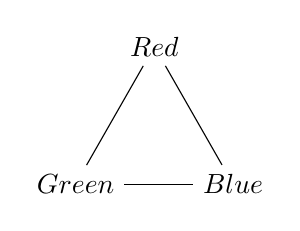
\begin{tikzpicture}
  \node (B) at (2,0) {$Red$};
  \node (D) at (1,-1.75) {$Green$};
  \node (E) at (3,-1.75) {$Blue$};

  \draw (D) -- (E);
  \draw (D) -- (B);
  \draw (E) -- (B);
\end{tikzpicture}
\end{center}


and the instance graph is literally just the problem graph with no modification. As we can see, the CSP problem can be formulated in a completely non-syntactic manner; without variables or clauses and such. It is a purely graph-theoretic problem, though it is not always helpful to think of it as such. Graph coloring, because it's already about graphs, is quite naturally expressed in these terms. Since the CSP and the model graph are the same, we can identify each graph with a CSP over a single binary relation. In particular, the complete graph of size k corresponds to the model graph for k-coloring.

To generalize to binary CSPs with multiple relations, we must switch to an edge-colored graph. 

\begin{definition}
Fix a set of colors, $C$. An edge-$C$-colored graph is a set of vertices, $V$, and a set of ordered pairs indexed by $C$, $\{E_i\}_{i\in C}$, representing an edge with an associated color. 
\end{definition}

\begin{definition}
An edge-$C$-colored graph homomorphism from a graph $G = (V_G, \{E_{G,i}\}_{i\in C})$ to a graph $H = (V_H, \{E_{H, i}\}_{i\in C})$ is a function $f_V: V_G \rightarrow V_H$ that satisfies the following condition:
\begin{equation}
    \forall c \in C, (u, v) \in E_{G, c}, \quad (f_V(u), f_V(v)) \in E_{H, c}.    
\end{equation}    
\end{definition}

This means that the function $f$ preserves the edge and color structure of the graph. In other words, edge-connected vertices in $G$ are always mapped to edge-connected vertices in $H$ of the same color.

This definition does allow for parallel edges, but such edges must be of distinct colors.

To translate a problem into this framework, we can follow a similar procedure to before, merely noting that each distinct relation gets mapped to a distinct color. 2-SAT provides a good example of a problem fitting in this framework. We can characterize the three relations as three edge colors. The model graph will have two nodes, for $0$ and $1$, and every true instance for each relation will become an edge. If we assign the color red to $x \vee y$, blue to $\neg x \vee y$, and green to $\neg x \vee \neg y$, we get the following model graph

\begin{center}
\begin{tikzpicture}[>=stealth, auto, node distance=2cm]

% Nodes
\node (0) at (0,0) {0};
\node (1) at (2,0) {1};

% Blue arrows
\draw [->, blue] (0) to [out=270, in=205, looseness=8] (0);
\draw [->, blue] (1) to [out=90, in=20, looseness=8] (1);
\draw [->, blue] (0) -- (1);

% Red arrows
\draw [->, red] (1) to [out=270, in=335, looseness=8] (1);
\draw [<->, red] (0) to [out=320, in=220] (1);

% Green arrows
\draw [->, darkgreen] (0) to [out=90, in=160, looseness=8] (0);
\draw [<->, darkgreen] (0) to [out=40, in=140] (1);

\end{tikzpicture}
\end{center}

Note that parallel edges of the same color going in opposite directions have been consolidated into two-headed arrows for conciseness. The 2-SAT problem can be recast as the goal of finding a homomorphism into this graph from an instance graph. Going back to our example from \ref{sec:two-sat}, we can turn it into the instance graph.

\begin{center}
\begin{tikzpicture}[>=stealth, auto, node distance=2cm]

% Nodes
\node (x1) at (0,0) {$x_1$};
\node (x2) at (2,0) {$x_2$};
\node (x3) at (1,1.5) {$x_3$};

% Blue arrows
\draw [->, blue] (x2) -- (x1);
\draw [->, blue] (x1) -- (x3);
\draw [->, blue] (x3) -- (x2);

% Green arrow
\draw [->, darkgreen] (x1) to [out=320, in=220] (x2);

\end{tikzpicture}
\end{center}

The model graph representation allows us to more efficiently reason about the problem. The cycle of blue arrows can only be mapped onto a self-loop by any homomorphism, meaning that all variables must be mapped to the same point. Further, the green arrow must then be mapped onto a self-loop, the only green one being at $0$, allowing us to rapidly conclude the same mapping we found by resolution earlier.
% This loop-based reasoning is a common solving technique and will be expanded upon in section \ref{sec:equality-detection}.

We may also give a graphical interpretation of resolution, at least in this restricted case. The existence of a parallel green and blue arrow forces us to assign $0$ to the variable at the source of the blue arrow. This comes from the fact that all parallel green and blue arrows of the model graph have $0$ in the source of the blue arrow. Similarly, a parallel red and blue arrow forces us to assign $1$ to the variable at the target of the blue arrow. Also, a parallel red and green arrow forces us to conclude that the variables are not equal, though it does not force a specific assignment on its own.

In order to capture all CSPs, we must generalize to edge-colored hypergraphs. 

\begin{definition}
Fix a set, $C$, of colors, and an arity-function, $a$, mapping $C$ to $\mathbb{N}^*$, the non-zero natural numbers. An edge-$(C, a)$-colored hypergraph is a set of vertices, $V$, and a set of ordered $a(c)$-tuples indexed by $c \in C$, $\{E_i\}_{i\in C}$, representing a hyper-edge with an associated color. 
\end{definition}

\begin{definition}
An edge-$(C, a)$-colored hypergraph homomorphism from a hypergraph $G = (V_G, \{E_{G,i}\}_{i\in C})$ to a hypergraph $H = (V_H, \{E_{H, i}\}_{i\in C})$ is a function $f_V: V_G \rightarrow V_H$ that satisfies the following condition:
\begin{equation}
    \forall c \in C, t \in E_{G, c}, \quad \prod_{i<a(c)} f_V(t_i) \in E_{H, c}.    
\end{equation}
Where $\prod_{i<n}$ is used to construct an n-tuple.
\end{definition}

The translation should be obvious at this point. The domain becomes the set of vertices, relations become colors, and the arity of the colors is the same as the arity of their relation.

At this point, drawing the model graph explicitly becomes unwieldy. 3-SAT has three colors, each with 7 hyper-edges, and several with self-loops of some kind. Many common ways of drawing hypergraphs don't support self-loops and the ones that do create a quite unreadable representation. I will not try to draw an example, as a consequence, but this completes our presentation of CSPs in terms of graph homomorphism. What I've called edge-colored hypergraphs are usually called "relational structures" in the CSP literature \citep{feder1998computational}. That is the terminology I'll use for the rest of this survey.

\begin{remark}\label{remark:just-graphs}
It was noted earlier that 3-coloring is an NP-complete problem. It was also noted that all finite-domain CSPs are, at most, NP-hard. This means we can translate all CSPs into graph homomorphism problems efficiently, eliminating the need for colors or hyper-edges in the process. However, such representations are far less direct than the colored hyper-graphs mentioned here. There is a trade-off in conceptual simplicity in exchange for sticking to a more familiar setting.
\end{remark}

Representing the model graph directly is generally only feasible for small, finite-domain CSPs. CSPs over large domains, such as those over large finite fields, will have model graphs proportional to the size of their domain, which can be extremely large. As such, implicit representations would have to be used.

It should also be noted that our definitions do not restrict ourselves to the finite domain. Infinite graphs, such as the Rado graph, can also be interpreted as CSPs without conceptual difficulty.